\documentclass{article}
\usepackage[utf8]{inputenc}
\usepackage[russian]{babel}
\usepackage{amsmath,amssymb,amsfonts}
\usepackage{geometry}

\geometry{a4paper, margin=3cm} 

\usepackage{booktabs}
\usepackage{tabularx}

\usepackage{graphicx}
\usepackage{cite}

\DeclareMathOperator{\sech}{sech}

\begin{document}

\section{Модель}

Распространение огибающих оптических импульсов в легированном эрбием волокне (EDF) описывается системой связанных уравнений Гинзбурга–Ландау для двух поляризационных компонент \(u(z,t)\) и \(v(z,t)\) \cite{main}:

\begin{equation}
    f(u, v) = \frac{i\Delta\beta}{2}u - \delta\frac{\partial u}{\partial t} - \frac{i\beta_2}{2}\frac{\partial^2 u}{\partial t^2} +
    \frac{g}{2}u + \frac{g}{2\Omega_g^2}\frac{\partial^2 u}{\partial t^2} +
    i\gamma\left(|u|^2 + \frac{2}{3}|v|^2\right)u + \frac{i\gamma}{3}v^2 u^*,
\end{equation}

\begin{equation}
    \begin{cases}
        \frac{\partial u}{\partial z} = f(u, v), \\
        \frac{\partial v}{\partial z} = f(v, u)
    \end{cases}
\end{equation}

Здесь \(z\) --- расстояние распространения, \(t\) --- время в сопутствующей системе отсчета.

Систему (1) удобно записать в операторном виде \(\partial_z \mathbf{w} = (\hat L + \hat N)\mathbf{w}\), где \(\mathbf{w}=(u,v)^T\), линейный оператор

\begin{equation}
    \hat L = \left(\frac{i\Delta\beta}{2} + \frac{g}{2}\right) - \delta\,\partial_t + \left(\frac{g}{2\Omega_g^2} - \frac{i\beta_2}{2}\right)\partial_t^2,
\end{equation}

а нелинейный оператор

\begin{equation}\label{eq:nonlin_ode}
    \hat N\begin{pmatrix}u\\v\end{pmatrix} =
    i\gamma \cdot \begin{pmatrix}
        \Bigl[\bigl(|u|^2+\tfrac{2}{3}|v|^2\bigr)u + \tfrac{1}{3}v^2 u^*\Bigr] \\[4pt]
        \Bigl[\bigl(|v|^2+\tfrac{2}{3}|u|^2\bigr)v + \tfrac{1}{3}u^2 v^*\Bigr]
    \end{pmatrix}.
\end{equation}

Физический смысл параметров:

\begin{table}[h!]
    \centering
    \renewcommand{\arraystretch}{1.3} % Чуть больше воздуха в строках
    \begin{tabularx}{\textwidth}{@{} >{\raggedright\arraybackslash}p{2.5cm} >{\raggedright\arraybackslash}X >{\raggedright\arraybackslash}X @{}}
        \toprule
        Параметр        & Смысл                                   & Роль в расщеплении                                                                                \\
        \midrule
        \(\beta_2\)     & групповая дисперсия (ГВД)               & определяет баланс с нелинейностью; знак \(\beta_2\gamma<0\) нужен для светлых солитонов           \\
        \(\gamma\)      & керровская нелинейность                 & \textbf{главный «руль» расщепления}: при росте \(|\gamma|\) импульс выходит из баланса и излучает \\
        \(\Delta\beta\) & линейное двулучепреломление             & связь между поляризациями, влияет на векторные моды                                               \\
        \(\delta\)      & параметр задержки/потерь                & входит в условие существования точного решения                                                    \\
        \(g\)           & усиление (\(g>0\)) или потери (\(g<0\)) & диссипация; при \(g\neq0\) точных sech-решений нет                                                \\
        \(\Omega_g\)    & полоса усиления                         & спектральная фильтрация                                                                           \\
        \bottomrule
    \end{tabularx}
\end{table}

Для наблюдения расщепления ключевым является \textbf{выход из баланса «дисперсия ↔ нелинейность»}. Практически это достигается варьированием:

\begin{itemize}
    \item \(|\gamma|\) --- увеличение сверх значения, при котором начальное условие является точным солитоном (основной сценарий);
    \item начальной амплитуды/ширины импульса (через \(\xi_1\)) при фиксированных параметрах среды;
    \item относительной фазы \(\psi_0\) между \(u\) и \(v\) (максимальный энергообмен при \(\psi_0=\pi/4\)).
\end{itemize}

\section{Численная схема}

Используем \textbf{метод расщепления (split-step)} с \textbf{симметричным расщеплением Стренга}. Шаг по \(z\) реализуется как

\begin{equation}
    \mathbf{w}(z+\Delta z) \approx e^{\frac{\Delta z}{2}\hat L}\, e^{\Delta z\, \hat N}\, e^{\frac{\Delta z}{2}\hat L}\, \mathbf{w}(z).
    \tag{5}
\end{equation}

\begin{itemize}
    \item \textbf{Линейный полушаг} \(e^{\frac{\Delta z}{2}\hat L}\) равносилен умножению в Фурье пространстве на \(\exp[\tilde L(\omega)\,\Delta z/2]\), где
          \begin{equation}
              \tilde L(\omega) = \frac{g}{2} - \frac{g}{2\Omega_g^2}\omega^2 + i\left(\frac{\Delta\beta}{2} - \delta\,\omega + \frac{\beta_2}{2}\omega^2\right).
          \end{equation}
    \item \textbf{Нелинейный полный шаг} \(e^{\Delta z\,\hat N}\) интегрируется методом Рунге--Кутты 4-го порядка (РК4) по \(z\) в каждой точке сетки по \(t\).
\end{itemize}

Использование пространства Фурье позволяет весьма точно считать производные по времени, но влечет периодические граничные условия по \(t\).

\section{Обоснование порядка точности}

Докажем, что схема Стренга имеет \textbf{второй порядок по \(\Delta z\)}.

\subsection{Разложение точного решения}

Точное решение на одном шаге разложим в ряд Тейлора по \(\Delta z\) (обозначим \(h=\Delta z\), все операторы действуют на \(\mathbf{w}_n=\mathbf{w}(z_n)\)):

\begin{equation}
    \begin{aligned}
        \mathbf{w}(z_n+h) = \mathbf{w}_n + h(\hat L+\hat N)\mathbf{w}_n + \frac{h^2}{2}(\hat L+\hat N)^2\mathbf{w}_n + O(h^3),                                                                                                \\
        \mathbf{w}(z_n+h) = \mathbf{w}_n + h\hat L\mathbf{w}_n + h\hat N\mathbf{w}_n + \frac{h^2}{2}\hat L^2\mathbf{w}_n + \frac{h^2}{2}(\hat L\hat N+\hat N\hat L)\mathbf{w}_n + \frac{h^2}{2}\hat N^2\mathbf{w}_n + O(h^3), \\
        \mathbf{w}(z_n+h) = \mathbf{w}_n + h \left(\hat L + \hat N \right) \mathbf{w}_n + \frac{h^2}{2}\left(\hat L^2 + \hat L\hat N+\hat N\hat L+ \hat N^2 \right)\mathbf{w}_n  + O(h^3).
    \end{aligned}
\end{equation}

\subsection{Разложение численного оператора}

Разложим экспоненты в (5):

\begin{equation}
    \begin{aligned}
        e^{\frac{h}{2}\hat L} = I + \frac{h}{2}\hat L + \frac{h^2}{8}\hat L^2 + O(h^3), \\
        e^{h\hat N} = I + h\hat N + \frac{h^2}{2}\hat N^2 + O(h^3).
    \end{aligned}
\end{equation}

Нелинейный подшаг \(e^{h\hat N}\mathbf{w}\) есть решение ОДУ \(\partial_z \mathbf{w} = \hat N(\mathbf{w})\) на шаге \(h\).
Классический РК4 имеет \textbf{локальную ошибку \(O(h^5)\)} и глобальную \(O(h^4)\), что на два порядка выше основного члена ошибки расщепления \(O(h^3)\).

Перемножая три оператора и сохраняя члены до \(h^2\) включительно:

\begin{itemize}
    \item члены \(O(1)\): \(I\);
    \item члены \(O(h)\): \(\frac{h}{2}\hat L + h\hat N + \frac{h}{2}\hat L = h\hat L + h\hat N\);
    \item члены \(O(h^2)\):
          \begin{itemize}
              \item \(\frac{h^2}{8}\hat L^2 + \frac{h^2}{4}\hat L^2 + \frac{h^2}{8} \hat L^2 = \frac{h^2}{2}\hat L^2\);
              \item \(\frac{h^2}{2}\hat L\hat N + \frac{h^2}{2}\hat N\hat L\);
              \item \(\frac{h^2}{2}\hat N^2\).
          \end{itemize}
\end{itemize}

Итого:
\begin{equation}
    \mathbf{w}_{n+1} = \mathbf{w}_n + h(\hat L+\hat N)\mathbf{w}_n + \frac{h^2}{2}\left[\hat L^2 + \hat L\hat N + \hat N\hat L + \hat N^2\right]\mathbf{w}_n + O(h^3).
    \tag{7}
\end{equation}

На полном интервале \(Z\) число шагов \(N = Z/h\), поэтому глобальная ошибка
\begin{equation}
    E_{\text{global}} = N (\mathbf{w}(z_n+h) - \mathbf{w}_{n+1}) = \frac{Z}{h}\cdot O(h^3) = O(h^2).
    \tag{9}
\end{equation}

Ключевой момент: второй порядок возникает \textbf{именно благодаря симметрии} расщепления (5). В несимметричной схеме Ли--Троттера \(e^{h\hat L}e^{h\hat N}\) в разложении появился бы член \(h^2\hat L\hat N\) без парного \(\hat N\hat L\), и компенсация в (7) нарушилась бы, что дало бы только первый порядок.

По переменной \(t\) метод является \textbf{спектральным} (производные в Фурье-пространстве вычисляются точно для разрешенных мод),
поэтому ошибка по \(\Delta t\) убывает быстрее любой степени при достаточном разрешении импульса.

% ----------------------------------------
% ----------------------------------------
% ----------------------------------------

\section{Тесты на порядок сходимости}

Для верификации численной схемы используем точное решение уравнения~\eqref{eq:CGLE} в форме светлого солитона~\cite[Eq.~40]{main}:
\begin{equation}\label{eq:bright_soliton}
    u(z, t) = A\,\operatorname{sech}\!\bigl(\eta\,(z - c_0\, t - w_0)\bigr)\;
    e^{\,i(k z - \omega t)},
    \qquad v(z,t) \equiv 0,
\end{equation}
где параметры огибающей определяются соотношениями~\cite[Eq.~39]{main}:
\begin{equation}\label{eq:eta_A}
    \eta^2 = -\xi_1, \qquad A^2 = -\frac{2\,\xi_1}{\xi_2},
\end{equation}
а коэффициенты $\xi_1$, $\xi_2$ выражаются через параметры модели~\cite[Eq.~10]{main}:
\begin{equation}\label{eq:xi}
    \xi_1 = \frac{\beta_2\,\omega^2 - 2\,\omega/c_0 + 2k - \Delta\beta}{\beta_2\,c_0^2},
    \qquad
    \xi_2 = -\frac{2\,\gamma}{\beta_2\,c_0^2}.
\end{equation}
Решение~\eqref{eq:bright_soliton} существует при условиях~\cite[Eq.~7,~41]{main}:
\begin{equation}\label{eq:conditions}
    \delta = \frac{1 - \beta_2\,c_0\,\omega}{c_0}, \qquad
    g = 0, \qquad \xi_1 < 0, \qquad \xi_2 > 0 \;\Leftrightarrow\; \beta_2\,\gamma < 0.
\end{equation}

Для тестов выбираем параметры, соответствующие рис.~11 из~\cite{main}:
\begin{equation}\label{eq:params}
    k = 13,\quad c_0 = 1.4,\quad \omega = 5,\quad w_0 = 0,
\end{equation}
\begin{equation}\label{eq:params_model}
    \Delta\beta = 25,\quad \beta_2 = 0.025,\quad \Omega_g = 10,\quad
    \gamma = -0.014,\quad g = 0.
\end{equation}

Точное решение~\eqref{eq:bright_soliton} удовлетворяет уравнению~\eqref{eq:CGLE} только при строгом выполнении условия~\eqref{eq:conditions} на параметр $\delta$. Подставляя значения~\eqref{eq:params}--\eqref{eq:params_model}:
\[
    \delta_{\mathrm{exact}}
    = \frac{1 - \beta_2\,c_0\,\omega}{c_0}
    = \frac{1 - 0.025 \cdot 1.4 \cdot 5}{1.4}
    = \frac{0.825}{1.4}
    = 0.589286\ldots
\]

Однако в ~\cite{main} указано $\delta = 0.59$.

\subsection{Мера ошибки}

Будем использовать в качестве меры ошибки следующие функционалы:

\begin{equation}
    \begin{aligned}
        \varepsilon_{abs} = \displaystyle\max_{z,\,t}\bigl|u_{\mathrm{num}}(z,t) - u_{\mathrm{an}}(z,t)\bigr|
        \varepsilon = \frac{\varepsilon_{abs}}{\displaystyle\max_{z,\,t}\bigl|u_{\mathrm{an}}(z,t)\bigr|}\;\times\; 100\;\%.
    \end{aligned}
\end{equation}

% ---------------------------------------
% ---------------------------------------
% ---------------------------------------
\section{Результаты верификации}

\subsection{Корректный параметр \(\delta = \delta_{\mathrm{exact}}\), непериодическое решение}

На рис.~\ref{fig:profile_correct} показано сравнение численного и аналитического профилей светлого солитона при $\delta = \delta_{\mathrm{exact}}$ на широкой непериодической сетке. Визуальное совпадение подтверждает корректность реализации схемы. На рис.~\ref{fig:convergence_correct} представлены результаты серии по $\Delta z$: наклон аппроксимирующей прямой $k \approx 2.0$ подтверждает второй порядок схемы Стренга.

\begin{figure}[htbp]
    \centering
    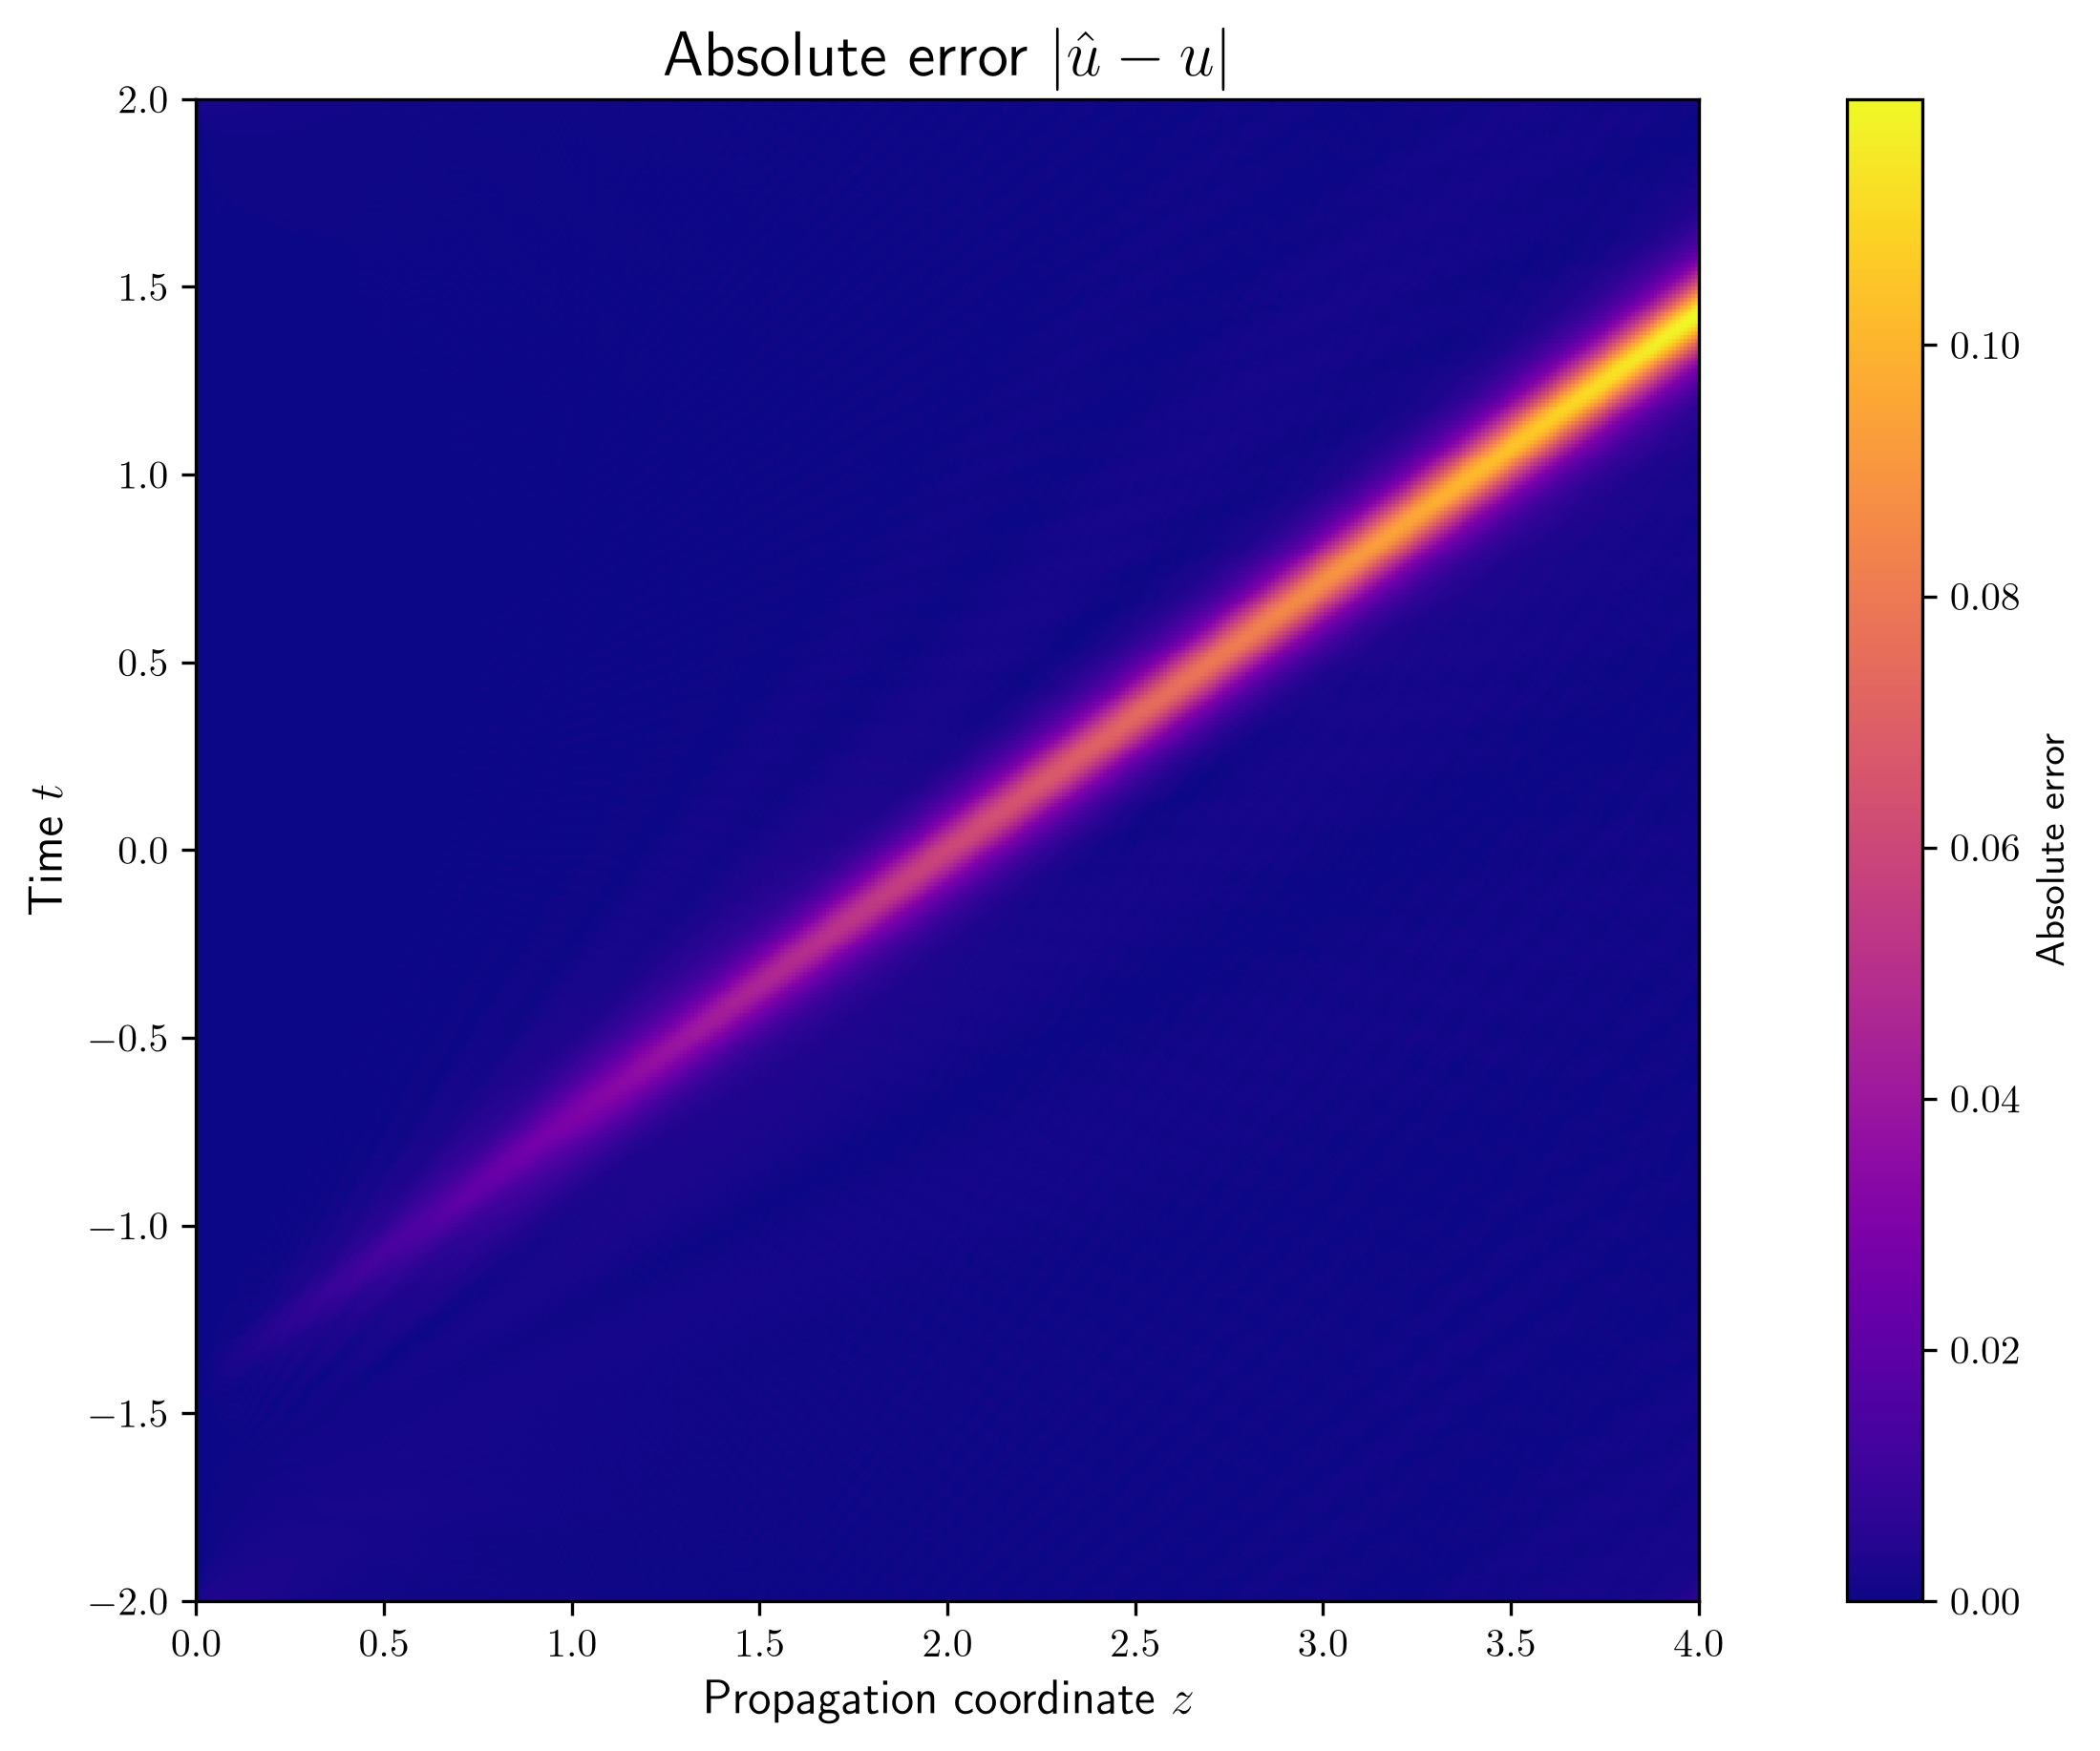
\includegraphics[width=0.85\textwidth]{figures/profile_delta_exact.png}
    \caption{Сравнение численного (сплошная линия) и аналитического (пунктир) профилей $|u(z,t)|$ при $\delta = \delta_{\mathrm{exact}} = 0.589286$, $z = z_{\max}$.
     Различия неразличимы в масштабе графика; максимальная относительная ошибка соответствует значению на рис.~\ref{fig:convergence_correct}.}
    \label{fig:profile_correct}
\end{figure}

\begin{figure}[htbp]
    \centering
    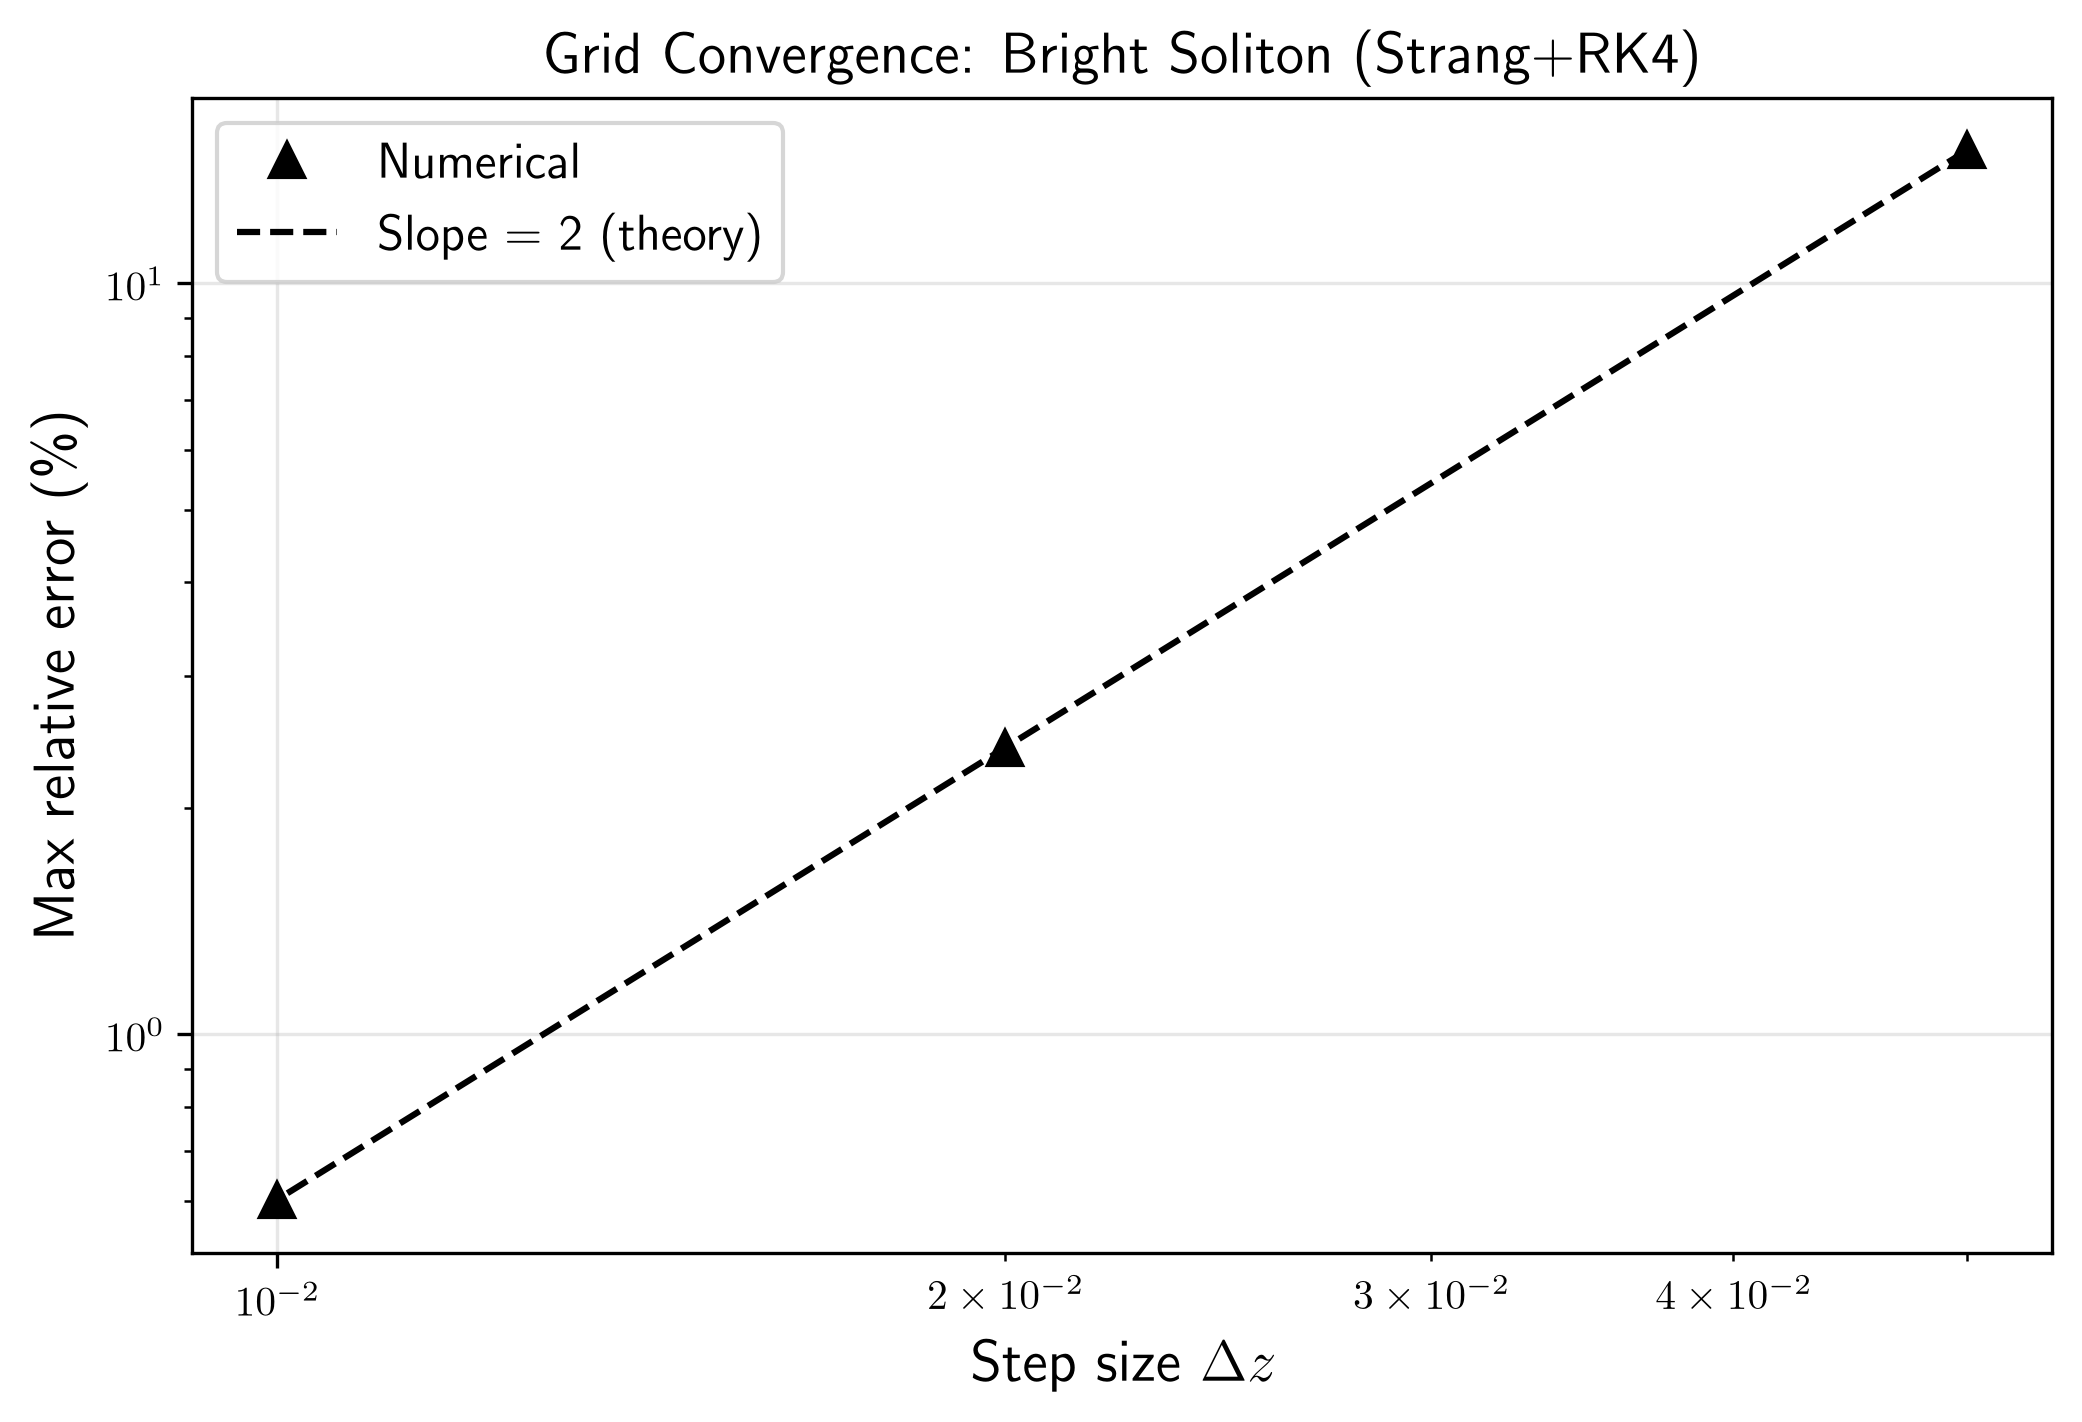
\includegraphics[width=0.85\textwidth]{figures/img_delta_ok.png}
    \caption{Сходимость по $\Delta z$ при $\delta = \delta_{\mathrm{exact}} = 0.589286$. Наклон аппроксимирующей прямой $k \approx 2.0$, что подтверждает второй порядок схемы Стренга по $\Delta z$.}
    \label{fig:convergence_correct}
\end{figure}

\subsection{Округлённый параметр \(\delta = 0.59\): деградация порядка}

На рис.~\ref{fig:convergence_rounded} представлены аналогичные результаты при $\delta = 0.59$ (значение из~\cite{main}). Ошибка содержит аддитивную составляющую $\varepsilon_{\mathrm{model}} \sim |R(\delta)|$, не зависящую от шагов сетки. При уменьшении $\Delta z$ ошибка выходит на плато, и наблюдаемый порядок стремится к нулю.

\begin{figure}[htbp]
    \centering
    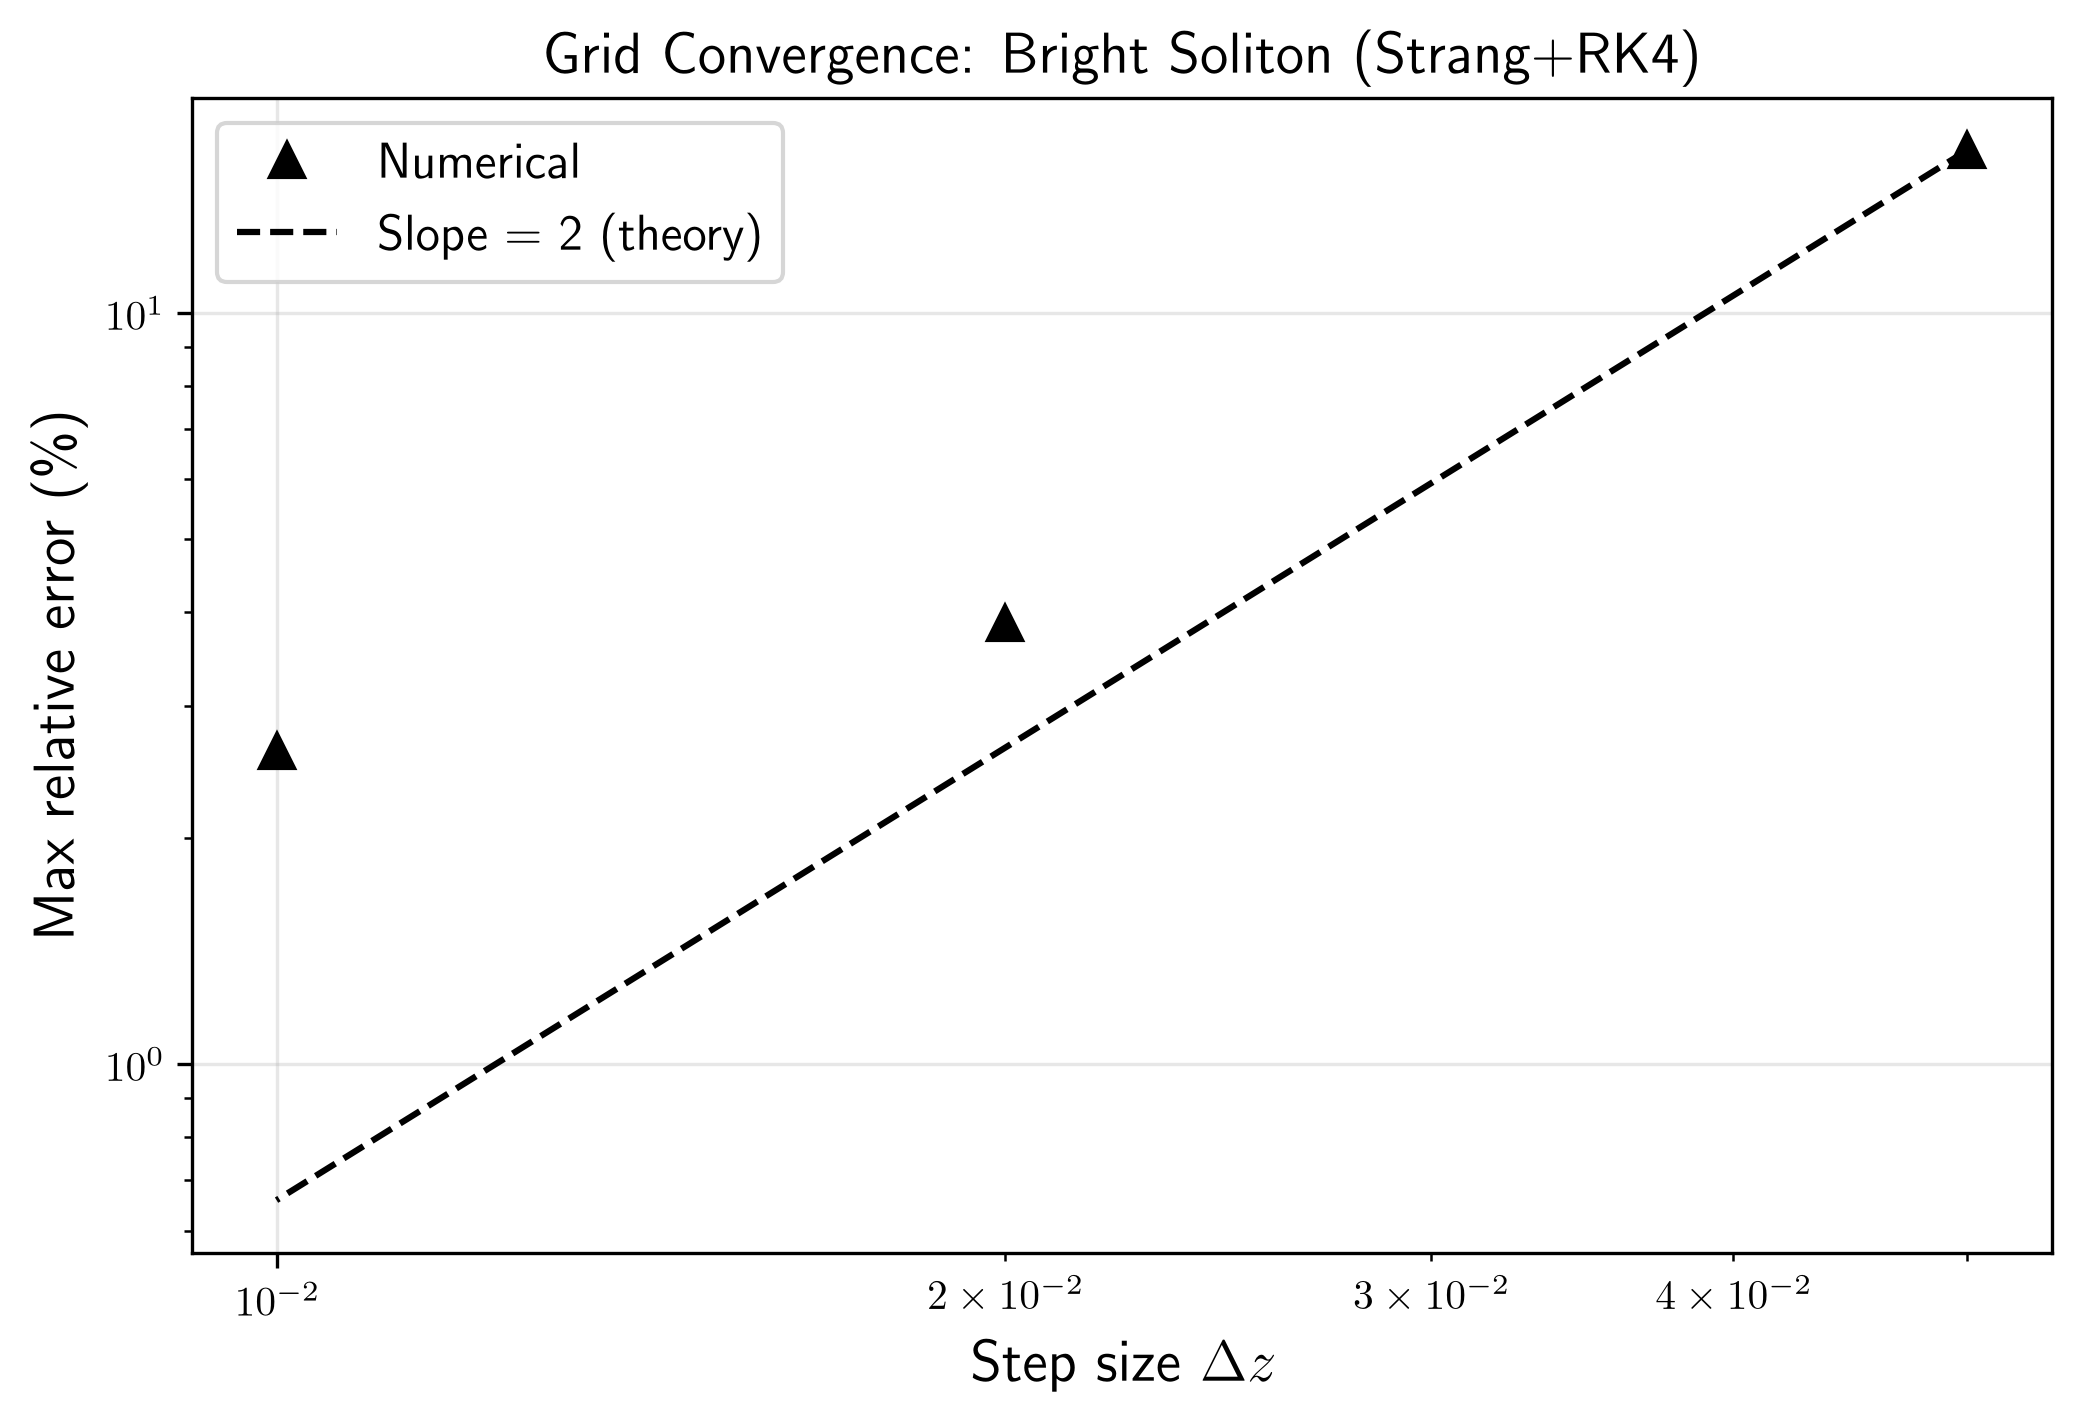
\includegraphics[width=0.85\textwidth]{figures/img_delta_br.png}
    \caption{Сходимость по $\Delta z$ при $\delta = 0.59$ (статья). Порядок сходимости нарушен: ошибка не убывает с теоретическим наклоном 2 из-за неустранимой составляющей, связанной с тем, что~\eqref{eq:bright_soliton} не является точным решением при данном $\delta$.}
    \label{fig:convergence_rounded}
\end{figure}

%====================================================================
\section{Проверка на зацикленной сетке}
%====================================================================

Солитон движется по времени со скоростью, определяемой \(c_0\): положение пика \(t_{\max}(z) = (z-w_0)/c_0\). За большое \(z\) пик смещается на величину, превышающую размер расчётного окна, поэтому применяются два подхода:
\begin{enumerate}
    \item \textbf{Большое окно} \(t \in [-T/2, T/2]\) с запасом, чтобы солитон не достигал границ. Периодические ГУ не влияют, ошибка определяется только схемой.
    \item \textbf{Зацикленная (подвижная) сетка}: окно малого размера, координата \(t\) циклически переставляется так, чтобы держать импульс в центре. Это позволяет моделировать большие \(z\) в компактном окне.
\end{enumerate}

\textbf{Наблюдение:} при одном и том же шаге \(\Delta t\) на зацикленной сетке присутствует дополнительная ошибка, которой \textbf{нет} на большом интервале \(t\).

\textbf{Причина:} циклический сдвиг массива выполняется на целое число узлов. Если истинное смещение пика за шаг \(\Delta z\) не кратно \(\Delta t\), возникает \textbf{субпиксельная ошибка представления} аналитического эталона на сетке (фактически ошибка интерполяции при сдвиге). Эта ошибка имеет порядок \(O(\Delta t)\) и не убывает при измельчении \(\Delta z\).

Ниже представлены три последовательных эксперимента, демонстрирующих природу этой ошибки.

\subsection{Большой интервал по \(t\): эталон без зацикливания}

На рис.~\ref{fig:cyclic_wide} показаны профиль решения и ошибка сходимости на широком временном окне (\(t \in [-80, 80]\), \(z \in [0, 50]\)). Солитон не достигает границ, периодические ГУ не активируются. Ошибка убывает с наклоном 2, как и ожидается для схемы Стренга.

\begin{figure}[htbp]
    \centering
    \begin{minipage}{0.48\textwidth}
        \centering
        \includegraphics[width=\textwidth]{figures/cyclic_wide_profile.png}
    \end{minipage}\hfill
    \begin{minipage}{0.48\textwidth}
        \centering
        \includegraphics[width=\textwidth]{figures/cyclic_wide_convergence.png}
    \end{minipage}
    \caption{Широкое окно (\(t \in [-80, 80]\)): (a) профиль \(|u(z,t)|\), солитон свободно движется без зацикливания; (b) сходимость по \(\Delta z\) с наклоном \(k \approx 2.0\). Эталонный случай.}
    \label{fig:cyclic_wide}
\end{figure}

\subsection{Уменьшение интервала по \(t\): появление зацикливания}

На рис.~\ref{fig:cyclic_narrow_coarse} показано то же решение на узком окне (\(t \in [-10, 10]\)) при том же шаге \(\Delta t = 0.021\). Солитон многократно пересекает границу и циклически переносится. На графике сходимости видно чёткое плато ошибки, не убывающее с \(\Delta z\). Порядок сходимости деградирует.

\begin{figure}[htbp]
    \centering
    \begin{minipage}{0.48\textwidth}
        \centering
        \includegraphics[width=\textwidth]{figures/cyclic_narrow_coarse_profile.png}
    \end{minipage}\hfill
    \begin{minipage}{0.48\textwidth}
        \centering
        \includegraphics[width=\textwidth]{figures/cyclic_narrow_coarse_convergence.png}
    \end{minipage}
    \caption{Узкое окно (\(t \in [-10, 10]\)), \(\Delta t = 0.021\): (a) профиль с видимыми артефактами зацикливания на границах; (b) сходимость по \(\Delta z\) с выходом на плато. Порядок падает из-за субпиксельной ошибки сдвига.}
    \label{fig:cyclic_narrow_coarse}
\end{figure}

\subsection{Уменьшение шага \(\Delta t\): восстановление порядка}

На рис.~\ref{fig:cyclic_narrow_fine} показано решение на том же узком окне (\(t \in [-10, 10]\)), но с уменьшенным шагом \(\Delta t = 0.005\). Субпиксельная ошибка сдвига уменьшается пропорционально \(\Delta t\), и плато опускается ниже уровня, ограничивающего сходимость при данном диапазоне \(\Delta z$. Наклон 2 восстанавливается в рабочем диапазоне шагов.

\begin{figure}[htbp]
    \centering
    \begin{minipage}{0.48\textwidth}
        \centering
        \includegraphics[width=\textwidth]{figures/cyclic_narrow_fine_profile.png}
    \end{minipage}\hfill
    \begin{minipage}{0.48\textwidth}
        \centering
        \includegraphics[width=\textwidth]{figures/cyclic_narrow_fine_convergence.png}
    \end{minipage}
    \caption{Узкое окно (\(t \in [-10, 10]\)), \(\Delta t = 0.005\): (a) профиль без видимых артефактов; (b) сходимость по \(\Delta z\) с восстановленным наклоном \(k \approx 2.0\). Уменьшение \(\Delta t\) подавляет ошибку субпиксельного сдвига.}
    \label{fig:cyclic_narrow_fine}
\end{figure}

\subsection{Ошибка взятия модуля}

При вычислении ошибки как \(\bigl||u_{\mathrm{num}}| - |u_{\mathrm{an}}|\bigr|\) вместо \(|u_{\mathrm{num}} - u_{\mathrm{an}}|\) теряется информация о фазовой ошибке. Для светлого солитона фаза набегает линейно по \(z\), и даже малая фазовая рассинхронизация между численным и аналитическим решениями приводит к тому, что ошибка модуля \textbf{систематически занижает} истинную ошибку. На рис.~\ref{fig:modulus_error} показано сравнение двух мер ошибки.

\begin{figure}[htbp]
    \centering
    \includegraphics[width=0.85\textwidth]{figures/modulus_error_comparison.png}
    \caption{Сравнение полной ошибки \(|u_{\mathrm{num}} - u_{\mathrm{an}}|\) (тёмные маркеры) и ошибки модуля \(\bigl||u_{\mathrm{num}}| - |u_{\mathrm{an}}|\bigr|\) (светлые маркеры). Ошибка модуля занижает истинную погрешность и может маскировать проблемы с фазовой согласованностью схемы.}
    \label{fig:modulus_error}
\end{figure}

\textbf{Вывод по верификации.} Для корректной проверки порядка сходимости необходимо:
\begin{enumerate}
    \item использовать \(\delta = \delta_{\mathrm{exact}}\);
    \item проводить тест на непериодической (достаточно широкой) временной сетке;
    \item использовать полную комплексную ошибку, а не ошибку модуля;
    \item при работе с зацикленной сеткой контролировать, чтобы \(\Delta t\) был достаточно мал для подавления субпиксельной ошибки сдвига.
\end{enumerate}

%====================================================================
\section{Спектральный анализ и конфигурации для исследования расщепления}
%====================================================================

\subsection{Спектры Фурье}

Расщепление импульса сопровождается генерацией новых спектральных компонент. Мониторинг спектра \(|\tilde u(\omega, z)|^2\) позволяет выявить начало расщепления раньше, чем оно станет заметно во временной области. Характерные признаки:
\begin{itemize}
    \item уширение спектра и появление боковых лепестков --- начало модуляционной неустойчивости;
    \item формирование отдельных спектральных пиков --- разделение импульса на суб-импульсы;
    \item рост низкоамплитудного фона вдали от несущей частоты --- излучение дисперсионных волн.
\end{itemize}

\begin{figure}[htbp]
    \centering
    \begin{minipage}{0.48\textwidth}
        \centering
        \includegraphics[width=\textwidth]{figures/spectrum_stable.png}
    \end{minipage}\hfill
    \begin{minipage}{0.48\textwidth}
        \centering
        \includegraphics[width=\textwidth]{figures/spectrum_splitting.png}
    \end{minipage}
    \caption{Эволюция спектра \(|\tilde u(\omega, z)|^2\): (a) стабильный солитон (\(\gamma = \gamma_{\mathrm{ref}}\)), спектр сохраняется; (b) режим расщепления (\(\gamma = 2\gamma_{\mathrm{ref}}\)), видны боковые пики и рост дисперсионного фона.}
    \label{fig:spectra}
\end{figure}

\subsection{Конфигурации параметров для исследования расщепления}

На основе анализа~\cite{main} (раздел 4.2, рис.~13--14) предлагаются следующие конфигурации для систематического исследования расщепления. Базовые параметры солитона соответствуют рис.~14 из~\cite{main}:
\[
    k = 12.8,\quad c_0 = 1.5,\quad \omega = 4.2,\quad w_0 = 0,\quad
    \beta_2 = 0.04,\quad \Omega_g = 10,\quad \Delta\beta = 21,\quad g = 0.
\]
Начальное условие: \(u(0,t)\) --- светлый солитон~\eqref{eq:bright_soliton} с \(\gamma_{\mathrm{ref}} = -0.01\); \(v(0,t) = 0.1\,e^{i\pi/4}\,u(0,t)\) (максимальный энергообмен согласно~\eqref{eq:energy_exchange}).

\begin{table}[htbp]
    \centering
    \renewcommand{\arraystretch}{1.3}
    \begin{tabular}{llp{7cm}}
        \hline
        \textbf{Конфигурация} & \textbf{Параметр} & \textbf{Ожидаемый эффект} \\
        \hline
        A (эталон)   & \(\gamma = \gamma_{\mathrm{ref}} = -0.01\)     & Стабильный солитон, осцилляции энергии без расщепления \\
        B (порог)    & \(\gamma = -0.02\)                              & Начало излучения дисперсионных волн (рис.~14a~\cite{main}) \\
        C (расщепление) & \(\gamma = -0.04\)                           & Выраженное расщепление + сильное излучение (рис.~14b~\cite{main}) \\
        D (фаза)     & \(\psi_0 = 0\) вместо \(\pi/4\)                 & Нет энергообмена, расщепление подавлено \\
        E (амплитуда)& \(v(0,t) = 0.5\,e^{i\pi/4}u(0,t)\)             & Усиленный энергообмен, более раннее расщепление \\
        F (дисперсия)& \(\beta_2 = 0.02\) вместо \(0.04\)              & Изменение баланса дисперсия/нелинейность, сдвиг порога \\
        G (усиление) & \(g = 0.1,\ \Omega_g = 10\)                     & Диссипативный режим, стабилизация или дестабилизация солитона \\
        \hline
    \end{tabular}
    \caption{Матрица конфигураций для исследования расщепления импульсов.}
    \label{tab:splitting_configs}
\end{table}

Рекомендуемая последовательность исследований:
\begin{enumerate}
    \item Воспроизвести конфигурации A--C, подтвердить качественное соответствие рис.~13--14 из~\cite{main}.
    \item Построить карту режимов в плоскости \((|\gamma|, \psi_0)\) при фиксированных остальных параметрах.
    \item Исследовать влияние амплитуды затравки (конфигурация E) на порог расщепления.
    \item Перейти к диссипативному случаю (конфигурация G) и изучить конкуренцию усиления и расщепления.
\end{enumerate}

\begin{figure}[htbp]
    \centering
    % \includegraphics[width=0.85\textwidth]{figures/regime_map.pdf}
    \fbox{\parbox{0.85\textwidth}{\centering\vspace{2cm}
            [Рисунок: карта режимов в плоскости \((|\gamma|, \psi_0)\).\\
                Области: стабильный солитон / осцилляции / расщепление / излучение.]
            \vspace{2cm}}}
    \caption{Карта динамических режимов связанной системы УГЛ. Границы определяются балансом нелинейности, межмодового обмена и дисперсии.}
    \label{fig:regime_map}
\end{figure}

% \section{Следующие шаги}

% \begin{itemize}
%     \item Воспроизвести распространение светлого солитона + график ошибки по \(z\).
%     \item Провести серии сходимости (раздел 4), подтвердить наклон 2 по \(\Delta z\).
%     \item Перейти к исследованию расщепления: воспроизвести сценарий с \(\gamma_{\text{ref}}=-0.01\), моделирование при \(\gamma=-0.02\) и \(-0.04\), затравка \(v(0,t)=0.1\,e^{i\pi/4}u(0,t)\).
%     \item Построить карты режимов в плоскости \((\gamma, \text{амплитуда})\) для поиска порога расщепления.
% \end{itemize}

\begin{thebibliography}{9}
    \bibitem{main} Название статьи. Численное исследование связанных уравнений Гинзбурга–Ландау: аналитические решения, схема Стренга, энергообмен между компонентами.
\end{thebibliography}

\end{document}